\section{Aussagenlogik}

\begin{frame}{Aussagenlogik}
	Aussagen sind Sätze, die entweder \textbf{wahr} oder \textbf{falsch} sind.\\
	Deren Wahrheitswert muss dabei nicht unbedingt bekannt oder \enquote{tatsächlich ermittelbar} sein.
	
	\pause
	\begin{Beispiel}
		\begin{itemize}
			\item „$ 1 + 1 = 2 $“ ist eine Aussage. Sie ist wahr.
			\item \enquote{Es gibt nur endlich viele Primzahlen.} ist eine Aussage. Sie ist falsch.
			\pause
			\item Die Goldbachsche Vermutung (Jede gerade Zahl größer 2 ist Summe zweier Primzahlen) \pause ist eine Aussage. Ihr Wahrheitswert ist unbekannt.
			\pause
			\item „Die Welt wird am 11.11.11111 untergehen.“ \pause ist auch eine Aussage. Wir werden ihren Wahrheitswert aber wohl niemals ermitteln können.
			\pause
			\item \enquote{Gelb} ist keine Aussage.
			\pause
			\item \enquote{Dieser Satz ist falsch.} \pause ist keine Aussage. Dem Satz kann offensichtlich kein Wahrheitswert zugeordnet werden.
		\end{itemize}
	\end{Beispiel}
\end{frame}

\begin{frame}{Zwei Grundsätze der Aussagenlogik}
	
	\begin{itemize}
		\pause
		\item[1.] Jede Aussage ist \textbf{entweder} falsch \textbf{oder} wahr.\\
		Wir schreiben im Folgenden $\BB= \{\W, \F\}$
		\pause
		\item[2.] Der Wahrheitswert einer \textbf{zusammengesetzten} Aussage ist durch die
		Wahrheitswerte der \textbf{Teilaussagen} eindeutig festgelegt. \\
		\enquote{$2 + 2 = 5 \; \bimp \; \text{Pinguine können fliegen}$} ist \textbf{wahr}.\\[0.2em]
		%TODO
		%Ex falso quodlibet
	\end{itemize}

	\impl Weg vom Inhalt und betrachte stattdessen \textbf{Aussagevariablen}.
\end{frame}

\begin{frame}{Syntax}
	\begin{Definition}
		$Var_{AL}$ ist die Menge aller \textbf{Aussagevariablen}. \\
		Wir bilden aussagenlogische Formeln als Wörter über dem Alphabet $A_{AL} = \{ \bleftBr, \brightBr, \bnot, \bund, \boder, \bimp \} \cup Var_{AL}$ 
	\end{Definition}
	\pause
	\begin{Definition}
		$For_{AL}$ ist die Menge aller \textbf{syntaktisch korrekten Formeln} über $Var_{AL}$.\\
		\medskip
		(VL: induktive Definition über Konstruktionsabbildungen) \\
		Klammern, die überflüssig sind, können weg. Wir lesen es dann wie gewohnt (\enquote{ \bnot} vor \enquote{ \bund} vor \enquote{ \boder} vor \enquote{ \bimp}  {\small \#PunktVorStrichUndSo}).
	\end{Definition}
	\pause
	\begin{Beispiel}
		$$Var_{AL} = \{A, B, C\}$$
		$$For_{AL} = \set{(A  \bimp B) \boder \bnot B \bund C, \ C \bimp (\bnot C), ...}$$
	\end{Beispiel}
\end{frame}

\begin{frame}{Semantik}
	Die Semantik einer aussagenlogischen Formel wird durch ihre \textbf{Auswertung} bestimmt.\\
	Hierbei werden den Operatorsymbolen aus $A_{AL}$ boolesche Funktionen zugeordnet.
	
	\pause
	\begin{Definition}
		Eine \textbf{boolesche Funktion} ist eine Abbildung der Form
		$f \from \BB^n \functionto \BB$.
	\end{Definition}

	\pause
	\begin{Beispiel}
		\enquote{Handelsübliche} boolesche Funktionen sind  $b_{\bnot}$,
		$b_{\bund}$, $b_{\boder}$ und $b_{\bimp}$. 
	\end{Beispiel}
\end{frame}

\begin{frame}{Semantik}
	\let\w\W
	\let\f\F
	\begin{center}
		\begin{huge}
			$$\only<1-2|handout:1>{\bnot}\only<3-4|handout:2>{\bund}\only<5-6|handout:3>{\boder}\only<7-8|handout:4>{\bimp}$$
		\end{huge}
		Wahrheitstabelle: \\
		\medskip
		\only<1-2|handout:1>{
			\begin{tabular}{|c|c|}
				\hline 
				$A$ &  $\bnot A$ \\
				\hline
				\w & \uncover<2|handout:1>{\f} \\
				\hline
				\f & \uncover<2|handout:1>{\w} \\
				\hline
			\end{tabular}
		}
		\only<3-4|handout:2>{ 
			\begin{tabular}{|c|c|c|}
				\hline 
				$A$ & $B$ & $A \bund B$ \\
				\hline
				\w & \w & \uncover<4|handout:2>{\w} \\
				\hline
				\w & \f & \uncover<4|handout:2>{\f} \\
				\hline
				\f & \w & \uncover<4|handout:2>{\f} \\
				\hline
				\f & \f & \uncover<4|handout:2>{\f} \\
				\hline
			\end{tabular}
		}
		\only<5-6|handout:3>{ 
			\begin{tabular}{|c|c|c|}
				\hline 
				$A$ & $B$ & $A \boder B$ \\
				\hline
				\w & \w & \uncover<6|handout:3>{\w} \\
				\hline
				\w & \f & \uncover<6|handout:3>{\w} \\
				\hline
				\f & \w & \uncover<6|handout:3>{\w} \\
				\hline
				\f & \f & \uncover<6|handout:3>{\f} \\
				\hline
			\end{tabular}
		}
		\only<7-8|handout:4>{
			\begin{tabular}{|c|c|c|}
				\hline 
				$A$ & $B$ & $A \bimp B$ \\
				\hline
				\w & \w & \uncover<8|handout:4>{\w} \\
				\hline
				\w & \f & \uncover<8|handout:4>{\f} \\
				\hline
				\f & \w & \uncover<8|handout:4>{\w} \\
				\hline
				\f & \f & \uncover<8|handout:4>{\w} \\
				\hline
			\end{tabular}
		}
	\end{center}
\end{frame}

\begin{frame}{Semantik}
	Wenn wir den Wahrheitswert einer \textbf{zusammengesetzten} Aussage bestimmen wollen, brauchen wir die Werte der \textbf{verwendeten Aussagenvariablen}. \\
	\begin{Definition}
		Sei $V \subseteq Var_{AL}$ die Menge der verwendeten Aussagevariablen.\\
		Eine Funktion $I \from V \functionto \BB$ bezeichnet man als \textbf{Interpretation}.
	\end{Definition}
	
	

\end{frame}

\begin{frame}{Auswertung}
	\begin{Definition}
		Sei $I$ eine Interpretation. Dann liefert die Abbildung $val_I(A)$ den Wahrheitswert zu einer aussagenlogischen Formel $A$. \\
		\medskip
		Diese Funktion nennen wir \textbf{Auswertung} und berechnen sie schrittweise, z.~B.:
	\end{Definition}
	
	\begin{align*}
	&val_I((A \bimp B) \boder \bnot B)  \\
	\visible<2->{= \;&b_{\boder} (val_I(A\bimp B), val_I(\bnot B)) \\}
	\visible<3->{= \;&b_{\boder} (b_{\bimp} (val_I(A), val_I(B)), b_{\bnot}(val_I(B))) \\}
	\visible<4->{= \;&b_{\boder} (b_{\bimp} (I(A), I(B)), b_{\bnot}(I(B))) \\}
	\end{align*}
\end{frame}

\begin{frame}{Auswertung}
	\begin{Definition}
		Eine \textbf{Tautologie} ist eine aussagenlogische Formel, bei der für alle möglichen Interpretationen $I$ gilt: $val_I(A) = \W$. \\
		\impl Schreibweise: \quad $\models A$ \\
		\medskip
		
		\pause
		Zwei aussagenlogische Formeln $A$ und $B$ heißen \textbf{äquivalent}, wenn für jede beliebige Interpretation $I$
		$$val_I(A) = val_I(B)$$
		gilt. \\
		\impl Schreibweise: \quad $A \equiv B$
	\end{Definition}
\end{frame}

% TODO
\begin{frame}[t]{Auswertung}
	\only<all:1>{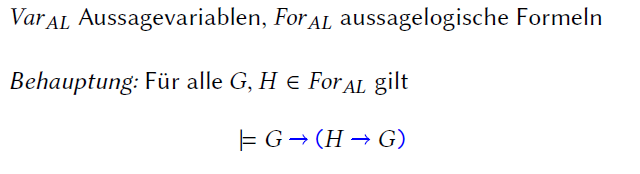
\includegraphics[scale=0.65]{al_uebung_1}\\[2em]
	Quelle: GBI-Übung 2015/2016}
	\only<all:2>{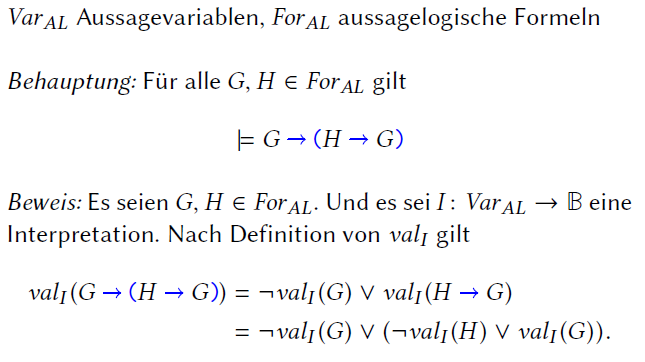
\includegraphics[scale=0.65]{al_uebung_2}}
	\only<all:3>{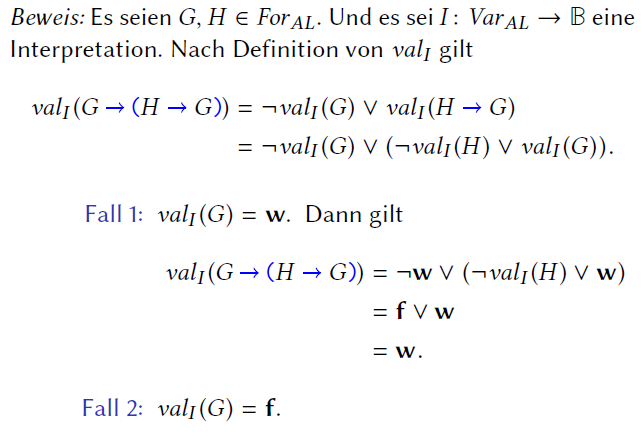
\includegraphics[scale=0.65]{al_uebung_3}}
	\only<all:4>{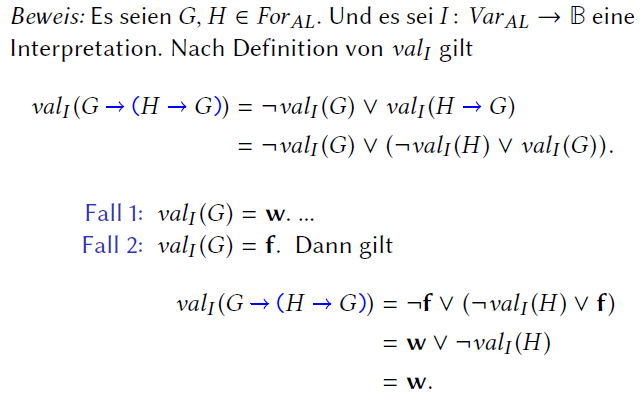
\includegraphics[scale=0.65]{al_uebung_4}}
	\only<all:5>{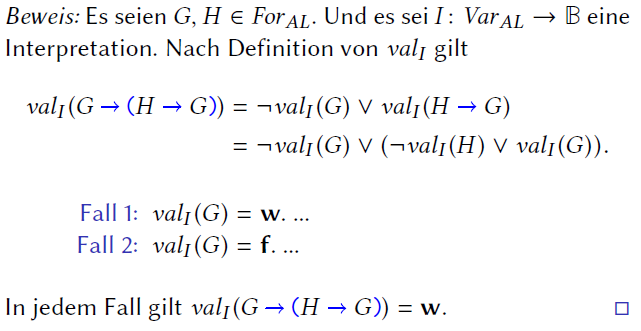
\includegraphics[scale=0.65]{al_uebung_5}}
\end{frame}

\begin{frame}{Semantik}
	
	Möchte man eine AL-Formel für alle möglichen Interpretationen auswerten, so macht man dies meist in Form einer \textbf{Wahrheitstabelle}.
	
	\begin{block}{Aufgabe}
		Gegeben seien die Formeln
		$$ F_1 = \left(\left(\left(B \bimp A \right) \boder B \right) \bimp (\bnot A)\right) \bund B$$
		und
		$$F_2 = \bnot A \bund B$$
		Stellt die Wahrheitstabellen von $F_1$ und $F_2$ auf. Sind die beiden Formeln äquivalent?
	\end{block}
\end{frame}

\begin{frame}{Lösung}
	Für die Formel $F_1$:
	\begin{table}[H]
	\centering
	\begin{tabular}{|*{6}{c|}}
	\hline
	$A$ & $B$ & $B \bimp A$ &  $\dots \boder B$ & $\dots \bimp \bnot A$ & $\dots \bund B$ \pause \\ \hline
	w & w & w & w & f & f  \\ \hline \pause
	w & f & w & w & f & f  \\ \hline \pause
	f & w & f & w & w & w  \\ \hline \pause
	f & f & w & w & w & f \\ \hline
	\end{tabular}
	\end{table}
\end{frame}

\begin{frame}{Lösung}
	Für die Formel $F_2$:
	\begin{table}[h!]
	\centering
	\begin{tabular}{|*{3}{c|}}
	\hline
	$A$ & $B$ & $\bnot A \bund B$  \\ \hline \pause
	w & w & f \\  \hline \pause
	w & f & f \\  \hline \pause
	f & w & w \\  \hline \pause
	f & f & f \\ \hline
	\end{tabular}
	\end{table}
	Also sind die beiden Formeln äquivalent: $$F_1 \equiv F_2$$
\end{frame}

\begin{frame}{Beweisbarkeit}
	Kalkül, Axiome, Schlussregeln, Modus Ponens, ...\\
	Siehe VL!
\end{frame}